\documentclass[11pt,a4paper]{article}

\usepackage[T1]{fontenc}
\usepackage[utf8]{inputenc}
\usepackage{lmodern}
\usepackage[margin=2.3cm]{geometry}
\usepackage{graphicx}
\usepackage{booktabs}
\usepackage{tabularx}
\usepackage{multirow}
\usepackage{amsmath,amssymb}
\usepackage{xcolor}
\usepackage{caption}
\usepackage{subcaption}
\usepackage{float}
\usepackage{enumitem}
\usepackage{tikz}
\usetikzlibrary{arrows.meta,positioning,fit,shapes.geometric}
\usepackage[colorlinks=true,linkcolor=blue!50!black,citecolor=blue!50!black,urlcolor=blue!50!black]{hyperref}

\graphicspath{{figures/}}
\setlist{itemsep=2pt,topsep=4pt}
\captionsetup{font=small,labelfont=bf}
\newcommand{\gco}{gCO$_2$}
\newcommand{\pp}{\,pp}

% ---------------------------------------------------------------- edit if needed
\newcommand{\institution}{[Department and Institution]}
% --------------------------------------------------------------------------------

\begin{document}

% ================================================================ title page
\begin{titlepage}
\centering
\vspace*{1.5cm}
{\Large 22AIE401 Reinforcement Learning \par}
\vspace{0.4cm}
{\large Project Report\par}
\vspace{1.6cm}
{\LARGE\bfseries PACE: Carbon- and SLA-Aware Edge--Cloud Task Scheduling with Deep Reinforcement Learning\par}
\vspace{0.6cm}
{\large Preference-conditioned, Adaptive, Carbon-aware Edge scheduler, evaluated in simulation and on a real AWS testbed\par}
\vspace{1.8cm}
{\large\bfseries Team\par}
\vspace{0.3cm}
\begin{tabular}{ll}
Nandu Manoj & CB.SC.U4AIE23321 \\
Naren Sundar L & CB.SC.U4AIE23322 \\
Vatturu Pardheev & CB.SC.U4AIE23344 \\
Charuvarthan T & CB.SC.U4AIE23359 \\
\end{tabular}
\vspace{1.4cm}

{\large\bfseries Guide\par}
\vspace{0.2cm}
{\large Dr.\ Palmani Duraisamy (Sr.\ Gd.)\par}
\vfill
{\large \institution\par}
\vspace{0.3cm}
{\large October 2026\par}
\end{titlepage}

% ================================================================ abstract
\begin{abstract}
\noindent
Edge--cloud platforms must decide, for every task of every job, whether to run it on a device at the edge, on a nearby fog server or in a distant cloud region. In India the nearby compute runs on one of the most carbon-intensive grids in the world, while clean grids such as Sweden's are 150--400\,ms away, so neither ``run local'' nor ``run green'' is right for every job.
Our base paper, MERSEM (Ramicetty et al., 2026), schedules whole jobs once per 15-minute epoch with an evolutionary search guided by tabular Q-learning, using a fixed weight between service-level (SLA) violations and carbon.
We present \textbf{PACE}, a deep reinforcement learning scheduler that places each ready task online in about 1\,ms. A single preference-conditioned policy, trained with behaviour cloning and PPO on domain-randomised simulations, covers the whole SLA--carbon trade-off through an input weight $w$. A PI controller adjusts $w$ at run time to hold an operator's SLA target, and a $w$-dependent safety shield removes placements that would clearly miss a deadline.
In simulation on the base paper's dataset (10 paired seeds), PACE misses 1.3\% of deadlines against MERSEM's 13.3\%, with 22\% less dynamic carbon ($p=0.002$), and it has the largest Pareto hypervolume. It keeps the lead under 2$\times$ load, runtime-estimate errors, node failures and rush hours, and on three of four setups it never saw during training.
We also built a real testbed with laptop edge workers in Coimbatore and EC2 instances in Mumbai and Stockholm. With an online network estimate, PACE missed fewer deadlines than MERSEM in all six paired runs ($-6.6$\pp, $p=0.031$) at a statistically insignificant +15\% carbon, and it matched the strongest heuristic (CA-EFT) on deadlines with 15\% less carbon ($p=0.031$).
We report three sim-to-real gaps the testbed exposed and how we fixed them, and we state the limitations honestly: larger analytics jobs, a much slower network than in training, and synthetic carbon-intensity profiles.
\end{abstract}

\tableofcontents
\newpage

% ================================================================ 1
\section{Introduction}

A smart-city platform runs three very different kinds of work on shared infrastructure. Cameras at junctions produce \emph{safety alerts} (for example a pedestrian in the lane) that must be detected within about one second. The city also runs \emph{graph analytics} over the road network, which need seconds and a lot of memory, and \emph{batch analytics} that only have to finish within hours. The compute is spread over three tiers: small devices at the edge, a fog server close by, and rented cloud capacity.

In our setting the edge is in Coimbatore, the fog is AWS Mumbai (about 30\,ms away but on a coal-heavy grid of roughly 650\,\gco/kWh), and the cloud is AWS Stockholm (about 150\,ms away, roughly 35\,\gco/kWh). Every placement is a trade-off between latency and carbon, and the right answer changes with load, the hour's grid carbon intensity, the network and node failures.

\paragraph{Why reinforcement learning.} Placement decisions are frequent and repetitive, so there is plenty of experience to learn from. The best action depends on a joint state that is hard to model by hand (queues, carbon, network, position in the job's DAG). The outcome (whether a job met its deadline) is only known later. Hand-made heuristics also have to be re-tuned whenever the objective or the conditions change. We still include a strong hand-tuned heuristic (carbon-aware earliest finish time, CA-EFT), so the learned policy has to earn its place.

\paragraph{Base paper.} MERSEM \cite{mersem} formulates exactly this problem (edge--fog--cloud, DAG jobs, SLA violations and carbon) and provides the dataset, system models and metrics we build on. It plans offline per 15-minute epoch, places whole jobs on one machine, uses a fixed weight between SLA and carbon, assumes perfect knowledge, has no failures and is evaluated in simulation only (Section~\ref{sec:base}).

\paragraph{Contributions.}
\begin{enumerate}
\item \textbf{Online, task-level placement} with a size-agnostic policy that scores each candidate node with a shared network, so it works for any number of nodes and simply masks failed ones.
\item \textbf{One preference-conditioned policy} for the whole SLA--carbon trade-off, plus an \textbf{online SLA-target controller} that tunes the preference at run time without retraining, and a \textbf{safety shield}.
\item \textbf{Robustness by design}: training with domain randomisation over topology, load, network and runtime-estimate noise; a deferral action for delay-tolerant work.
\item \textbf{Real-system evidence}: the same scheduler code runs in our simulator and on a real AWS + laptop testbed. We measure the sim-to-real gap, fix the three gaps it revealed, and report paired statistics.
\end{enumerate}

Each ingredient has precedents (Section~\ref{sec:related}); our contribution is their combination for carbon- and SLA-aware edge--cloud DAG scheduling, fixing the base paper's limitations, together with real-system validation.

% ================================================================ 2
\section{Background and related work}\label{sec:related}

\subsection{The base paper: MERSEM}\label{sec:base}
MERSEM \cite{mersem} schedules graph-analytics jobs in an edge--fog--cloud system. Once per 15-minute epoch, a workload predictor supplies the next epoch's jobs and a hybrid evolutionary algorithm searches for a job-to-machine mapping that minimises $w_s \cdot \text{SLA rate} + w_c \cdot \text{CO}_2$ with $w_s+w_c=1$. Tabular Q-learning chooses how strongly to perturb solutions in a local search (five actions, one step per episode). It is evaluated in an extended EdgeCloudSim \cite{edgecloudsim} on the Rezaee--Adabi DAG dataset \cite{dataset}.

Table~\ref{tab:critique} lists the assumptions we consider most limiting in practice and how PACE addresses each.

\begin{table}[H]
\centering\small
\caption{Main limitations of the base paper and how PACE addresses them.}
\label{tab:critique}
\begin{tabularx}{\textwidth}{>{\raggedright\arraybackslash}p{4.6cm}X}
\toprule
MERSEM assumption & PACE \\
\midrule
Offline batch plan per 15-min epoch from predicted arrivals & Online, event-driven decision per ready task in about 1\,ms \\
Whole job on one machine; jobs on a machine run sequentially & Task-level placement over the DAG; concurrent tasks with a measured contention model \\
Exact knowledge of runtimes, resources and carbon & Policy sees noisy estimates; noise is randomised during training \\
Fixed weight $w$ between a rate and grams of CO$_2$, three operating points & One policy for all $w$; a controller holds an SLA \emph{target} \\
No failures, stragglers or priority classes & Masking and re-placement of failed nodes' tasks; class priorities; deferral of batch work \\
The ``RL'' only tunes a perturbation rate; the search reruns every epoch & The RL agent \emph{is} the scheduler; decision cost is reported \\
Only metaheuristic baselines & EFT, carbon-greedy, tuned CA-EFT and MERSEM itself \\
Simulation only & Real AWS testbed with measured sim-to-real gap \\
\bottomrule
\end{tabularx}
\end{table}

While inspecting the dataset we found 51,895 jobs and 1,301,653 tasks (the paper mentions about half a million jobs), 7/16/62 tasks per job at the 10th/50th/90th percentile, and usable job-level deadlines. The ``real'' and ``predicted'' runtime columns are zero, so the dataset contains no estimate error; we inject it ourselves.

\subsection{RL lineage and related ideas}
DeepRM \cite{deeprm} showed online RL scheduling in a single cluster with REINFORCE; a follow-up added a behaviour-cloning warm start \cite{deeprm2}. We take the online decision process (several decisions at one instant with time frozen) from DeepRM and the warm start from its follow-up. Decima \cite{decima} scores DAG stages with a shared network; we use the same node-scoring idea in a geo-distributed setting with carbon and deadlines. Dependent-task offloading with deep RL \cite{wang2021} is close in spirit but has no carbon objective. Preference-conditioned multi-objective RL \cite{abels2019,yang2019} motivates a single policy conditioned on $w$, and PID Lagrangian methods \cite{stooke2020,ray2019} motivate our SLA controller. Carbon-aware temporal shifting \cite{wiesner2021} motivates the deferral action.

% ================================================================ 3
\section{Problem setting}\label{sec:problem}

\subsection{System}
The system has three tiers. \textbf{Edge} nodes are camera boxes in Coimbatore (grid zone IN-SO); each runs only its own jobs, one task at a time, at about 0.3$\times$ a cloud vCPU. \textbf{Fog} nodes are in AWS Mumbai (zone IN-WE). \textbf{Cloud} nodes are in AWS Stockholm (zone SE-SE3). Fog and cloud each have an x86 and an ARM machine with two vCPUs. Links between locations have a round-trip time and a bandwidth; every DAG edge whose endpoints run in different places pays RTT/2 plus size/bandwidth, and the result returns to the originating device.

\subsection{Jobs}
\begin{itemize}
\item \textbf{Class A, safety alerts}: a short camera pipeline (capture, detect, rules, alert) with a 1\,s deadline. About 30\% of camera feeds are privacy-restricted and may not leave India. Class A is about 98\% of all jobs.
\item \textbf{Class B, graph analytics}: DAGs from the base paper's dataset with deadline $2\cdot$(dataset slack ratio)$\cdot$(critical path)$+2$\,s.
\item \textbf{Class C, batch}: dataset DAGs with deadlines of 30 minutes to 2 hours; they may be deferred.
\end{itemize}
Jobs from the first 70\% of the dataset timeline are used for training and the last 30\% for testing. The held-out jobs are larger (median 25 vs 15 tasks), which matters in Section~\ref{sec:sim}.

\subsection{Energy and carbon}
Node power follows the Cloud Carbon Footprint method \cite{ccf}: idle and maximum watts per vCPU (x86 0.74/3.5\,W, ARM 0.47/1.69\,W) and a PUE of 1.135 for AWS. Carbon is energy times the hourly grid intensity of the node's zone (location-based accounting). We report \textbf{dynamic carbon}, the part a scheduler controls, as the primary carbon metric, and total carbon including idle power for comparability with MERSEM. Carbon-intensity traces are synthetic hourly profiles built from real annual means (IN-SO about 560, IN-WE about 680, SE-SE3 about 35\,\gco/kWh) with a daily solar dip, an evening peak and autocorrelated noise (Section~\ref{sec:limits}).

\subsection{Metrics}
The primary metric is the \textbf{SLA-violation rate} of classes A and B together (MERSEM's metric), reported per class as well, and dynamic carbon in grams. We also report the 95th-percentile alert latency, the share of work per tier, the decision time and the Pareto hypervolume (PHV) over (SLA rate, carbon), which MERSEM also uses.

% ================================================================ 4
\section{Method: PACE}\label{sec:method}

\begin{figure}[H]
\centering
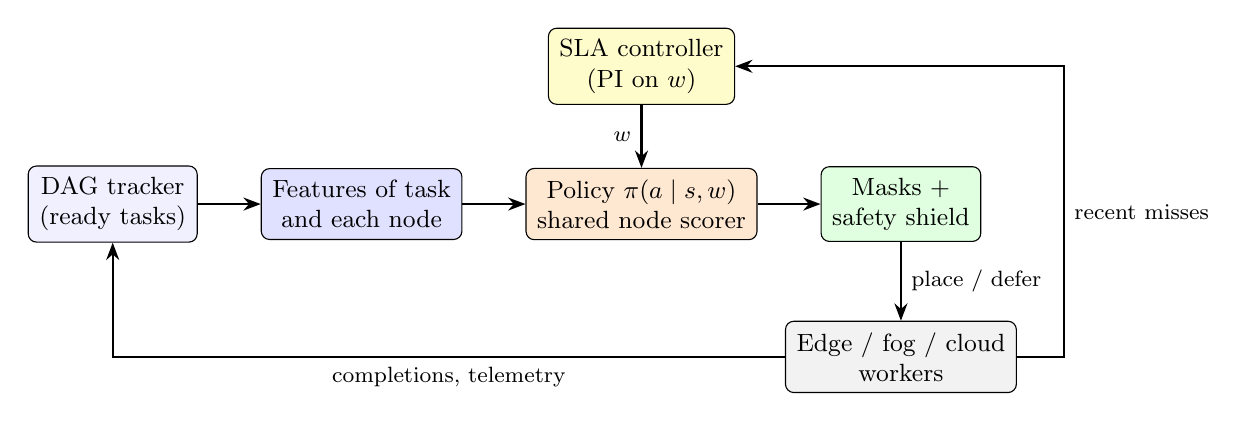
\begin{tikzpicture}[
  box/.style={draw,rounded corners=3pt,align=center,font=\small,minimum height=0.9cm,inner sep=4pt},
  arr/.style={-{Stealth[length=2.2mm]},thick}]
\node[box,fill=blue!6] (dag) {DAG tracker\\(ready tasks)};
\node[box,fill=blue!12,right=0.8cm of dag] (feat) {Features of task\\and each node};
\node[box,fill=orange!18,right=0.8cm of feat] (pol) {Policy $\pi(a\mid s,w)$\\shared node scorer};
\node[box,fill=green!12,right=0.8cm of pol] (shield) {Masks +\\safety shield};
\node[box,fill=gray!10,below=1.0cm of shield] (nodes) {Edge / fog / cloud\\workers};
\node[box,fill=yellow!20,above=0.8cm of pol] (ctrl) {SLA controller\\(PI on $w$)};
\draw[arr] (dag) -- (feat);
\draw[arr] (feat) -- (pol);
\draw[arr] (pol) -- (shield);
\draw[arr] (shield) -- node[right,font=\footnotesize]{place / defer} (nodes);
\draw[arr] (nodes.west) -| node[below,pos=0.25,font=\footnotesize]{completions, telemetry} (dag.south);
\draw[arr] (ctrl) -- node[left,font=\footnotesize]{$w$} (pol);
\draw[arr] (nodes.east) -- ++(0.6,0) |- node[right,pos=0.25,font=\footnotesize]{recent misses} (ctrl.east);
\end{tikzpicture}
\caption{PACE in the orchestrator. The same scheduler interface is used by the simulator and the real testbed.}
\label{fig:arch}
\end{figure}

\subsection{Decision process}
We model scheduling as a semi-Markov decision process. A decision epoch occurs whenever a task becomes ready (all parents finished), a deferred task wakes up, or a failure orphans tasks. When several tasks are ready at the same instant, they are decided one after another with time frozen, so the action space stays linear in the number of nodes.

\paragraph{Observation.} For the task (20 features): class, log estimated work, remaining critical path, time budget to its sub-deadline, slack ratio, deferral state, privacy flag, number of descendants, retry flag, the preference $w$, the recent SLA-violation rate, utilisation, time of day (sine/cosine), and two \emph{job-pressure} features (the job's remaining work relative to its time left and the server capacity). For each candidate node (18 features): tier, whether it is the origin device, speed, estimated transfer, wait, execution and finish time relative to the budget, carbon intensity now and the forecast change at +1\,h and +3\,h, the estimated carbon of this task relative to a reference, utilisation, queue length, and whether the estimated finish meets the budget (and 0.4$\times$ the budget). The job's DAG structure enters through the critical-path, descendant and job-pressure features; a full graph neural network encoder is future work.

\paragraph{Action and masks.} The action is a candidate node or \textsc{Defer}. Masks remove dead nodes, nodes without enough memory, cloud nodes for privacy-restricted tasks, other devices' edge nodes, and \textsc{Defer} unless the task is class C with enough slack and has been deferred fewer than three times.

\paragraph{Reward.} Each decision is rewarded for the task it placed:
\begin{equation}
r = -\Big[(1-w)\,\frac{c_{\text{task}}}{W_{\text{task}}\cdot \bar c_{\text{fog}}} \;+\; w\big(\tfrac12\,\ell_{\text{task}} + \tfrac12\,\ell_{\text{job}}\big)\Big],
\qquad \ell = \mathbb{1}[\text{late}]\Big(1+\min\big(1,\tfrac{\text{lateness}}{\text{window}}\big)\Big),
\end{equation}
where $c_{\text{task}}$ is the task's carbon, $W_{\text{task}}$ its work, $\bar c_{\text{fog}}$ the carbon per unit work on the fog (a normaliser that makes $w$ meaningful), $\ell_{\text{job}}$ the job's lateness penalty and $\ell_{\text{task}}$ the penalty against the task's \emph{sub-deadline}: the job deadline minus the task's estimated remaining critical path. This deadline decomposition was the key to credit assignment in large DAGs (Section~\ref{sec:history}). We use $\gamma=0.8$ and GAE $\lambda=0.9$, a short horizon because a decision is judged mainly by its own job.

\subsection{Network}
The policy applies one shared MLP (two hidden layers of 128 units) to the concatenation of each node's features and the task features, and a linear layer turns each node's embedding into a score. A separate small head scores \textsc{Defer}. The critic reads the task features plus the max- and mean-pooled node embeddings. Because the same scorer is applied to every node, the network has about 60\,K parameters regardless of the topology, and a failed node is simply masked out. Inference takes about 0.55\,ms on one CPU core.

\subsection{Training}
\begin{enumerate}
\item \textbf{Behaviour cloning} for three iterations on CA-EFT's decisions, so PPO starts near a good heuristic.
\item \textbf{Preference-conditioned PPO} \cite{ppo} (learning rate $3\cdot10^{-4}$, four epochs per iteration, masked logits) with $w\sim U[0,1]$ sampled per episode, so one network learns the whole trade-off.
\item \textbf{Domain randomisation} per episode: 2--6 edge, 1--3 fog and 1--3 cloud nodes, server speeds $\pm$20\%, RTT $\times$0.7--1.5, bandwidth $\times$0.5--1.5, alert rate 0.1--0.4 per camera per second, analytics load proportional to the server count, and runtime-estimate noise $\sigma\in[0,0.4]$.
\end{enumerate}
The final model was trained for 82 PPO iterations (about 3.5\,M decisions, 35 minutes on the laptop's CPU with parallel rollout workers). Figure~\ref{fig:training} shows the learning curves.

\begin{figure}[H]
\centering
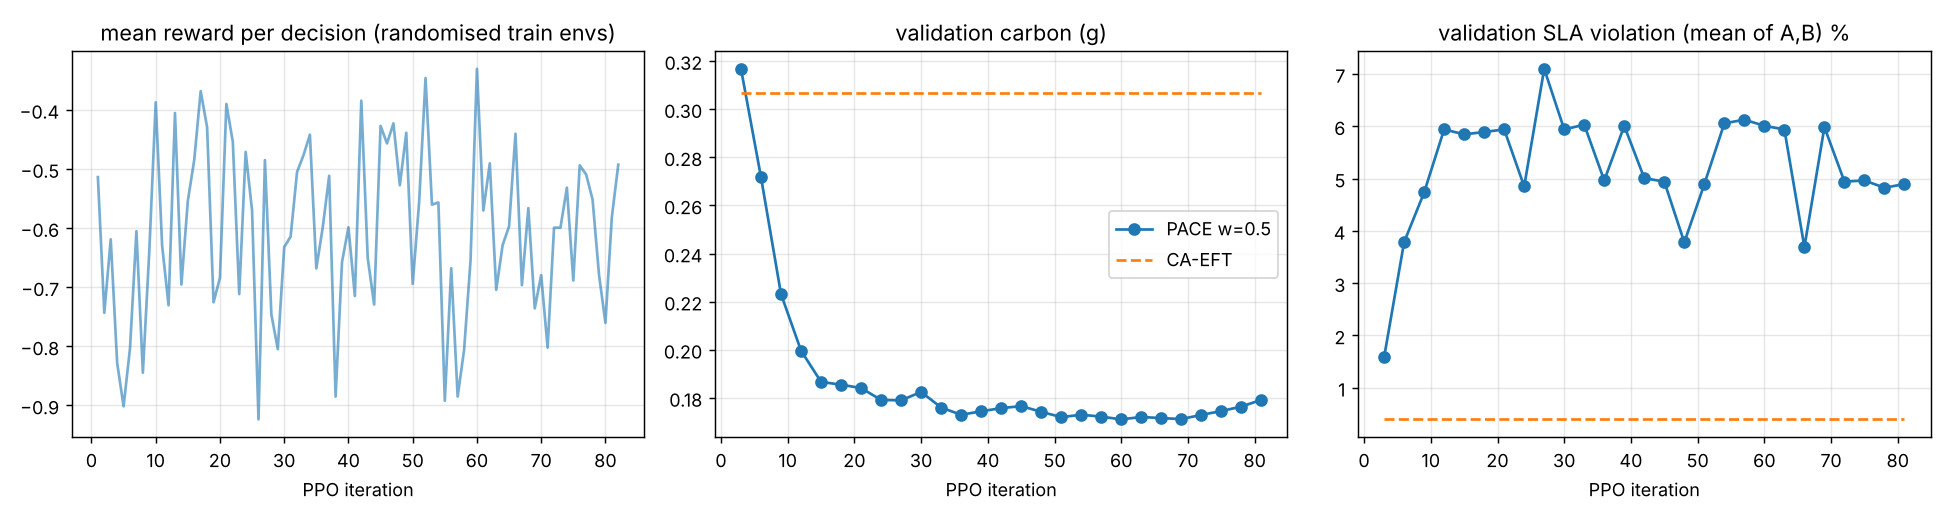
\includegraphics[width=\textwidth]{training.png}
\caption{Training of the final policy: mean reward per decision, and validation carbon and SLA violations against CA-EFT.}
\label{fig:training}
\end{figure}

\subsection{SLA-target controller and safety shield}
Because $w$ is an input, changing it changes the behaviour instantly. Every ten completed class A/B jobs, a PI controller compares the recent miss rate (window of 50 jobs) with the operator's target $\varepsilon$:
\begin{equation}
e = \text{miss rate} - \varepsilon,\qquad I \leftarrow \text{clip}(I+e,-5,5),\qquad w = \text{clip}(w_0 + 0.8\,e + 0.08\,I,\;0,\;1).
\end{equation}
This is the deployment-time analogue of a Lagrange multiplier on the SLA constraint. When the operator changes the target, the integral is reset so that $w$ reacts immediately (an anti-windup fix found during the demo rehearsal).

The \textbf{safety shield} removes nodes whose estimated finish exceeds a fraction of the task's budget that depends on $w$: 0.4 of the budget at $w=1$ and the full budget at $w=0$. If no node is safe, the shield abstains. The policy still chooses among the remaining nodes.

\subsection{Development history}\label{sec:history}
The first reward split the job penalty across its tasks; the policy ignored $w$ and missed 45\% of analytics deadlines on held-out data. Giving the full job penalty to every task (v2) still left credit unattributable for large DAGs. Deadline decomposition (v3) made $w$ matter. A class-balanced loss (v4) gave no gain. The final model (v5) adds the job-pressure features and class-priority queues on the nodes (alerts before analytics before batch), which we give to every method.

% ================================================================ 5
\section{Experimental setup}\label{sec:setup}

\paragraph{Simulator.} A custom discrete-event simulator models per-node execution slots with a contention slowdown, task-level transfers with log-normal jitter, the carbon and power models, failures and stragglers. Schedulers only see estimated runtimes. Two topologies are used: \emph{testbed} (2 edge, 2 fog, 2 cloud nodes, mirroring the real testbed) and \emph{city} (8 edge, 3 fog, 4 cloud nodes).

\paragraph{Baselines.} Random; edge-, fog- and cloud-only; carbon-greedy; EFT (earliest estimated finish); Job-EFT (whole job on the EFT node); \textbf{CA-EFT}, the greenest node whose estimated finish meets 0.4 of the task's budget, otherwise EFT (margin tuned on training seeds); and \textbf{MERSEM} with $w_s\in\{1,0.5,0\}$ (SLA, Balanced, Carbon) plus an oracle variant.

\paragraph{MERSEM re-implementation.} We follow the paper where it is specific: job-level placement with sequential jobs per machine, epoch planning, the weighted objective, a hybrid evolutionary algorithm with dominance-based replacement, and Q-learning-guided local search on 30\% of the population (10 episodes, 1 step each, $\alpha=0.15$, $\gamma=0.9$, five perturbation actions, the paper's reward). Unspecified choices are documented: population 20, 30 generations per epoch, uniform crossover. We are generous to it: its predictor sees the \emph{actual} next-epoch arrivals, its population is seeded with an EFT mapping, and unplanned or failed placements fall back to EFT immediately.

\paragraph{Protocol.} Every method sees the same jobs and carbon trace per seed (paired comparison), using the held-out test jobs only. E1 and E6 use 10 seeds and the stress tests 5. We report means with 95\% confidence intervals and test paired differences with the Wilcoxon signed-rank test. PACE runs at $w=0.9$ unless stated.

% ================================================================ 6
\section{Simulation results}\label{sec:sim}

\subsection{Nominal load (E1)}

\begin{table}[H]
\centering\small
\caption{E1, testbed topology, nominal load, 10 paired seeds (mean; 95\% CIs in the repository). Lower is better.}
\label{tab:e1}
\begin{tabular}{lrrrrr}
\toprule
Method & Alerts missed & Analytics missed & A+B missed & Dyn.\ carbon (g) & p95 alert (s) \\
\midrule
EFT & 10.4\% & 1.3\% & 10.3\% & 1.96 & 1.29 \\
Carbon-greedy & 65.8\% & 77.0\% & 66.0\% & 0.28 & 5.11 \\
CA-EFT & 2.8\% & 5.6\% & 2.8\% & 0.74 & 0.80 \\
MERSEM-SLA & 6.7\% & 33.6\% & 7.1\% & 1.82 & 1.31 \\
MERSEM-Balanced (base paper) & 12.7\% & 45.4\% & 13.3\% & 0.51 & 2.20 \\
MERSEM-Balanced, oracle & 10.7\% & 45.3\% & 11.3\% & 0.49 & 2.25 \\
\midrule
\textbf{PACE}, $w=0.9$ & \textbf{0.9\%} & 23.1\% & \textbf{1.3\%} & \textbf{0.39} & 0.84 \\
\textbf{PACE + shield}, $w=1$ & 1.8\% & 6.0\% & 1.9\% & 0.55 & 0.87 \\
PACE + shield, target 2\% & 1.8\% & 16.2\% & 2.1\% & 0.47 & 0.83 \\
\bottomrule
\end{tabular}
\end{table}

Against MERSEM-Balanced, PACE misses 12\pp\ fewer deadlines with 22\% less dynamic carbon, better in every seed ($p=0.002$ for both). Against the tuned CA-EFT it misses 1.5\pp\ fewer with 47\% less carbon ($p=0.01$ and $0.002$). On the larger city topology the gap to MERSEM is 17\pp\ and 34\% carbon (1.0\% vs 17.9\% missed).

\textbf{The weakness} is analytics jobs: pure PACE misses 23\% of them against CA-EFT's 5.6\%. Alerts are 98\% of the jobs, the held-out analytics DAGs are larger than the training ones, and the cost one placement imposes on other jobs is not in its own reward, so the policy overloads the small green cloud with large DAGs. The shield closes most of the gap (6.0\%).

\begin{figure}[H]
\centering
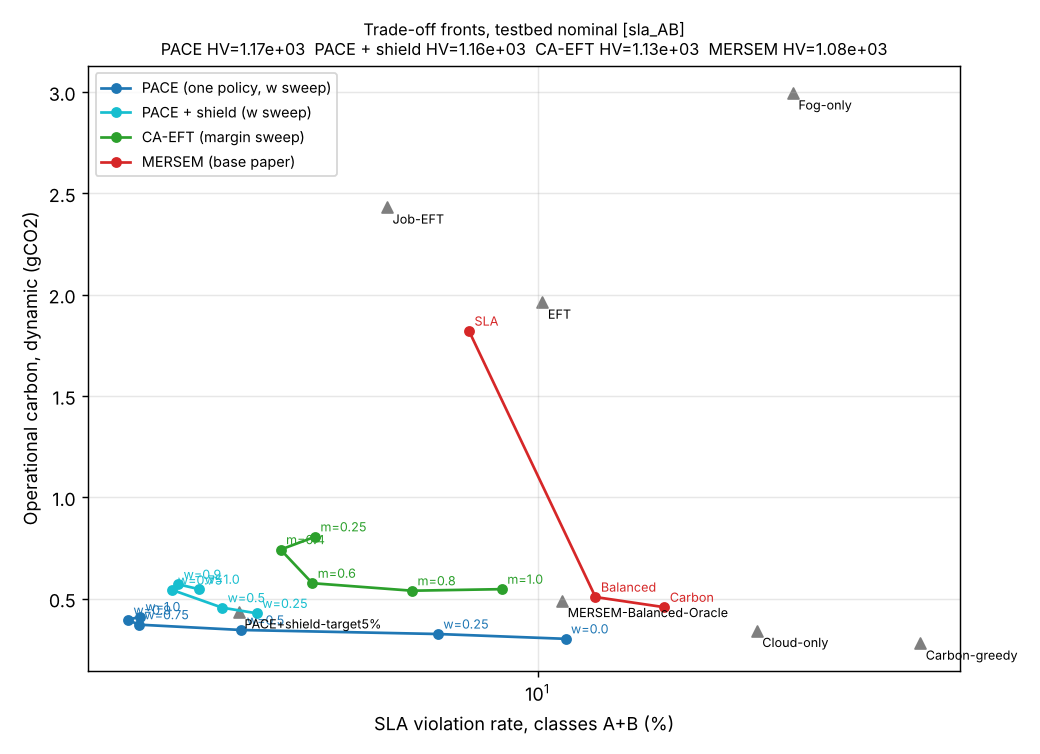
\includegraphics[width=0.85\textwidth]{pareto_testbed.png}
\caption{SLA--carbon trade-off on the testbed topology. One PACE policy sweeps $w$; CA-EFT sweeps its margin; MERSEM its three weights. Pareto hypervolume (higher is better): PACE 1172, PACE + shield 1156, CA-EFT 1131, MERSEM 1083. On the city topology: 2626, 2612, 2565 and 2287.}
\label{fig:pareto}
\end{figure}

\subsection{Stress tests (E2--E5)}

\begin{table}[H]
\centering\small
\caption{Deadlines missed (classes A+B) under stress, 5 paired seeds. Best per row in bold.}
\label{tab:stress}
\begin{tabular}{lrrrr}
\toprule
Scenario & MERSEM-Bal. & CA-EFT & PACE & PACE + shield \\
\midrule
1.5$\times$ load & 22.8\% & 4.5\% & \textbf{1.9\%} & 2.5\% \\
2$\times$ load & 26.3\% & 7.2\% & \textbf{3.0\%} & 4.8\% \\
Runtime estimates $\sigma=0.4$ & 14.0\% & 3.2\% & \textbf{1.2\%} & 1.4\% \\
Mumbai fog crash + stragglers & 26.4\% & 15.9\% & 14.8\% & \textbf{11.0\%} \\
Random failures (1 per node-hour) & 18.6\% & 4.0\% & \textbf{1.8\%} & 2.7\% \\
Rush hour ($\times$2.5 for 15 min)$^*$ & 22.0\% & 4.9\% & -- & \textbf{2.8\%} \\
\bottomrule
\end{tabular}

\smallskip\footnotesize $^*$ PACE + shield at $w=0.5$ in the rush-hour scenario; $w=0.9$ elsewhere.
\end{table}

A PACE variant has the fewest violations in every scenario, and PACE uses less dynamic carbon than CA-EFT in each one. PACE decides when each task is ready, so a crashed node is simply masked and its tasks re-placed; MERSEM plans per epoch and suffers most even with an immediate EFT fallback (Figure~\ref{fig:rush}).

\begin{figure}[H]
\centering
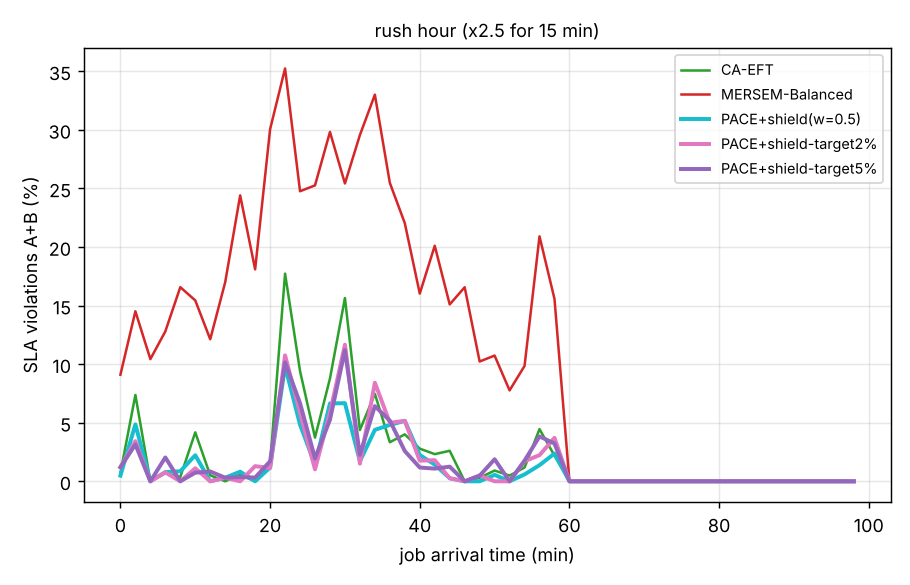
\includegraphics[width=0.75\textwidth]{e5_rush_hour.png}
\caption{Deadline misses over a one-hour run with a 15-minute rush hour starting at minute 20.}
\label{fig:rush}
\end{figure}

\subsection{Holding an SLA target}
With a 2\% target the controller achieved 2.0\% on the testbed topology and 1.7\% on the city. The value of $w$ each day settled at ranged from 0.25 to 0.87, adapting to that day's load and grid. A loose 5\% target gave 2.3\% violations and spent the headroom on carbon (25\% less than fixed $w=0.9$). A fixed-weight method like MERSEM can only reach a target by re-tuning and re-running its search.

\subsection{Generalisation to unseen setups (E6)}
We tested the trained policy, without any retraining, on four setups outside its training range (Table~\ref{tab:e6}). Running the larger city required one code change: the policy's node scorer is size-agnostic, but the implementation had a fixed buffer of 12 candidate nodes. The buffer now grows with the topology; the weights are unchanged, and results with 12 or fewer candidates are identical.

\begin{table}[H]
\centering\small
\caption{E6: deadlines missed (A+B), 10 paired seeds, city-scale load. PACE at $w=0.9$.}
\label{tab:e6}
\begin{tabular}{lrrr}
\toprule
Setup & PACE & CA-EFT & MERSEM-Bal. \\
\midrule
Seen: city, 8 edge / 3 fog / 4 cloud & \textbf{1.0\%} & 2.8\% & 17.9\% \\
2$\times$ larger city (16 / 6 / 8 nodes) & \textbf{0.4\%} & 4.6\% & 17.3\% \\
Cloud moved to Frankfurt (grid zone never seen) & \textbf{0.7\%} & 2.8\% & 16.2\% \\
2$\times$ heavier jobs, 3$\times$ more data & \textbf{2.7\%} & 7.6\% & 27.8\% \\
Slow WAN (RTT $\times$2, bandwidth $\times$0.3) & 17.3\% & \textbf{1.4\%} & 24.8\% \\
\bottomrule
\end{tabular}
\end{table}

On the first four setups PACE beats both baselines in 10 of 10 seeds ($p=0.002$) and uses less dynamic carbon than both (e.g.\ $-38\%$ vs MERSEM and $-44\%$ vs CA-EFT on the larger city). It \textbf{fails on the much slower WAN}: it keeps sending alerts to Stockholm, while CA-EFT simply recomputes finish times. This is the same weakness the real testbed exposed when the network drifted (Section~\ref{sec:real}); the remedies are an online network estimate and wider network randomisation in training.

\begin{figure}[H]
\centering
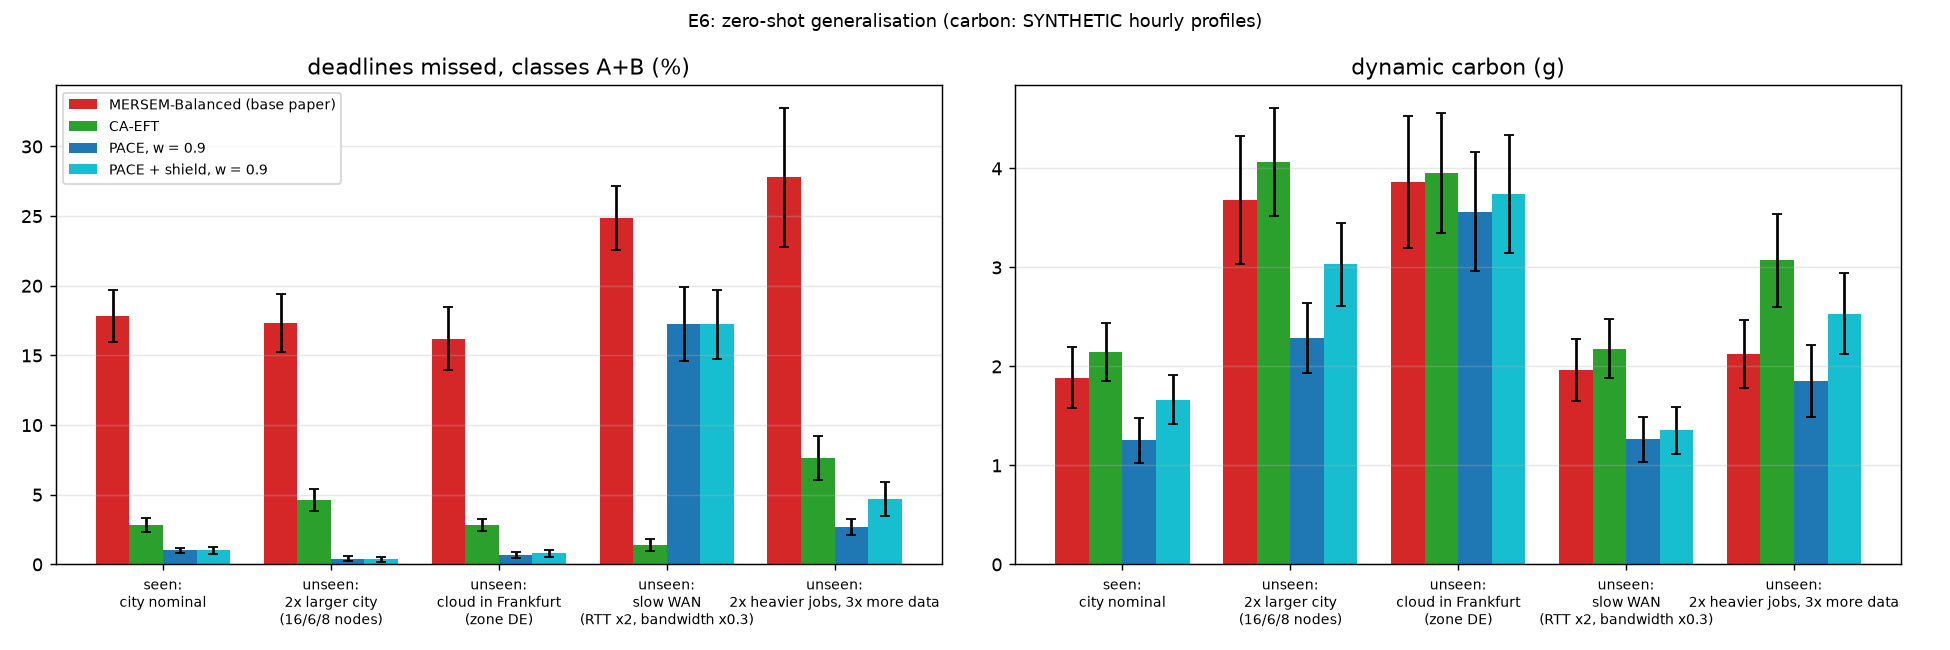
\includegraphics[width=\textwidth]{e6_generalisation.png}
\caption{E6: deadline misses and dynamic carbon on the seen setup and four unseen ones.}
\label{fig:e6}
\end{figure}

% ================================================================ 7
\section{Real AWS testbed}\label{sec:real}

\subsection{Setup}
Two laptop processes act as Pi-class edge camera boxes in Coimbatore (one core each, 3$\times$ slowdown). The fog is two EC2 instances in Mumbai (\texttt{c7i-flex.large} x86 and \texttt{t4g.small} ARM) and the cloud is the same pair in Stockholm. Workers run real tasks: a BLAS kernel for analytics work and OpenCV HOG pedestrian detection for camera frames. The orchestrator runs on the laptop with exactly the same scheduler code as the simulator, plus a live dashboard with buttons for node crashes, carbon spikes, rush hours and the SLA target. Each run lasts 6 minutes; schedulers are interleaved per seed (A B C D E, A B C D E, \ldots) so they share network conditions. PACE uses \texttt{pace\_live.pt}, the simulation policy fine-tuned in the calibrated digital twin (below).

\subsection{Calibration: closing three sim-to-real gaps}
A calibration script measures every node's speed per task type, the slowdown when all its cores are busy, and the RTT and bandwidth between the three locations. Configured with these measurements, the simulator becomes a \emph{digital twin} of the testbed, which we used to predict each experiment before running it. Smoke tests exposed three gaps:
\begin{enumerate}
\item \textbf{Dispatch.} The orchestrator held a core during a task's whole HTTP round trip, and the twin had no controller round trip. Tasks are now sent when placed, workers fetch inputs while others compute and start tasks by class priority, and the twin and every scheduler (MERSEM included) see the controller round trip.
\item \textbf{SMT contention.} A two-vCPU x86 instance is one physical core: two tasks at once each ran 1.7--1.8$\times$ slower, against 1.15$\times$ assumed; the ARM instances have two real cores and showed none. Calibration now measures the slowdown per node.
\item \textbf{Network drift} (next subsection).
\end{enumerate}
PACE was fine-tuned in three stages as the twin was corrected (about one hour on four CPUs); the checkpoint was chosen on training-split validation runs, not on the test seeds.

\subsection{E8: static network estimates}
In the first real experiment (5 schedulers $\times$ 3 seeds), alert misses were far above the twin's prediction for every scheduler, and PACE did not beat MERSEM overall (14.7\% vs 10.3\% missed), although it missed half as many analytics deadlines in every seed. The task records split each missed alert into network, queue and compute time: the queue was empty and compute took 0.03\,s; the loss was the \textbf{network time to Mumbai}, whose median grew from 0.25\,s to about 0.5\,s over the evening, independently of our traffic. PACE and CA-EFT ran most detections in Mumbai, trusting the calibrated 0.3\,s; MERSEM ran about 40\% on the edge and was less exposed.

\textbf{Fix: an online network estimate.} The orchestrator compares each task's measured network time with the calibrated model and adds the 90th percentile of the last 30 residuals per region to the latency estimate used by every scheduler, by PACE's features and by the shield. While the network is degraded, alerts then stay on the edge.

\subsection{E8b: with the online network estimate}

\begin{table}[H]
\centering\small
\caption{Real AWS testbed, E8b, 3 seeds per load. Missed = classes A+B. Carbon is dynamic operational carbon per 6-minute run.}
\label{tab:e8b}
\begin{tabular}{lrrrr}
\toprule
& \multicolumn{2}{c}{Nominal load} & \multicolumn{2}{c}{Busy hour (2$\times$ analytics)} \\
\cmidrule(lr){2-3}\cmidrule(lr){4-5}
Scheduler & Missed & Carbon (g) & Missed & Carbon (g) \\
\midrule
MERSEM-Balanced (base paper) & 9.4\% & 0.037 & 14.3\% & 0.063 \\
CA-EFT & 3.7\% & 0.051 & 6.2\% & 0.083 \\
EFT & 14.4\% & 0.282 & -- & -- \\
\textbf{PACE}, $w=0.9$ & 3.8\% & 0.044 & 6.6\% & 0.067 \\
\textbf{PACE + shield}, $w=0.9$ & 6.1\% & 0.050 & \textbf{4.6\%}$^\dagger$ & 0.069 \\
\bottomrule
\end{tabular}

\smallskip\footnotesize $^\dagger$ No alert deadlines missed. EFT at nominal load ran in a separate session after an orchestrator fix.
\end{table}

\begin{table}[H]
\centering\small
\caption{Paired comparison over the six E8b runs (3 nominal + 3 busy hour). Negative $\Delta$ = PACE better. With six pairs the smallest attainable Wilcoxon $p$ is 0.031.}
\label{tab:paired}
\begin{tabular}{llrrrrr}
\toprule
PACE variant & vs & Better in & $\Delta$ missed & $p$ & $\Delta$ carbon & $p$ \\
\midrule
PACE & MERSEM-Balanced & 6/6 & $-6.6$\pp & 0.031 & +15\% & 0.156 \\
PACE & CA-EFT & 2/6 & $+0.2$\pp & 0.875 & $-15\%$ & 0.031 \\
PACE + shield & MERSEM-Balanced & 4/6 & $-6.4$\pp & 0.156 & +25\% & 0.094 \\
PACE + shield & CA-EFT & 4/6 & $+0.4$\pp & 1.000 & $-9\%$ & 0.156 \\
\bottomrule
\end{tabular}
\end{table}

PACE missed fewer deadlines than MERSEM in all six paired runs, in both alerts and analytics, for 15\% more operational carbon on average (not significant). At $w=0.9$ PACE is configured to favour deadlines, while MERSEM-Balanced sits at a lower-carbon, higher-miss point, so neither dominates on both axes here. Against CA-EFT, PACE had the same deadline performance with 15\% less carbon. EFT, which ignores carbon, used about 6$\times$ PACE's carbon and missed more deadlines (Figure~\ref{fig:real}).

\begin{figure}[H]
\centering
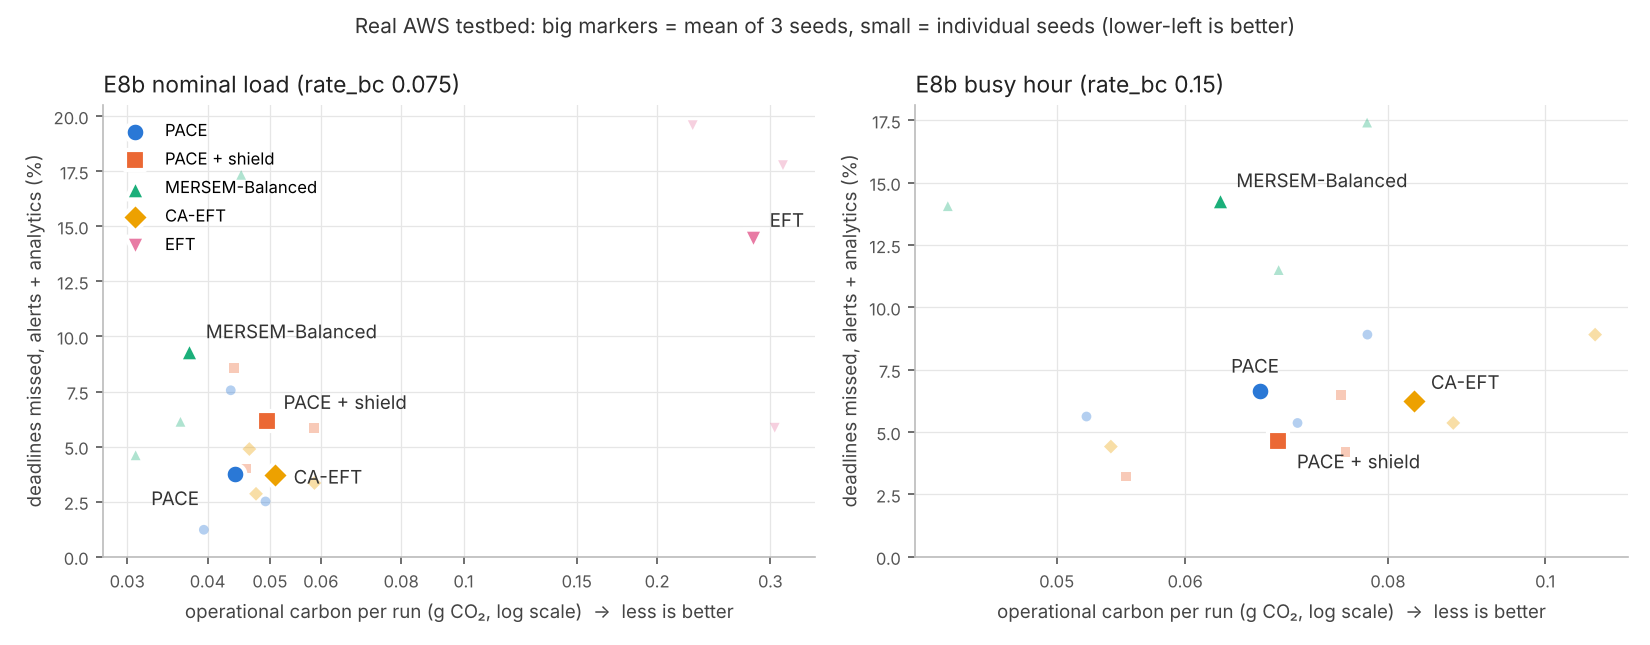
\includegraphics[width=\textwidth]{e8_real.png}
\caption{Real AWS testbed (E8b): deadlines missed against dynamic carbon at nominal load and in the busy hour.}
\label{fig:real}
\end{figure}

\subsection{Sim-to-real fidelity (E9)}
Replaying each real run's job trace in the twin shows that the twin is optimistic, mostly about alert latency: for example PACE + shield in the busy hour missed 6.5/4.2/3.2\% in reality against 6.5/3.8/2.4\% predicted, while at nominal load the real misses were several points higher than predicted. The remaining gap is mostly network-time variance on the campus uplink, which the twin's static link model underestimates (Figure~\ref{fig:e9}).

\begin{figure}[H]
\centering
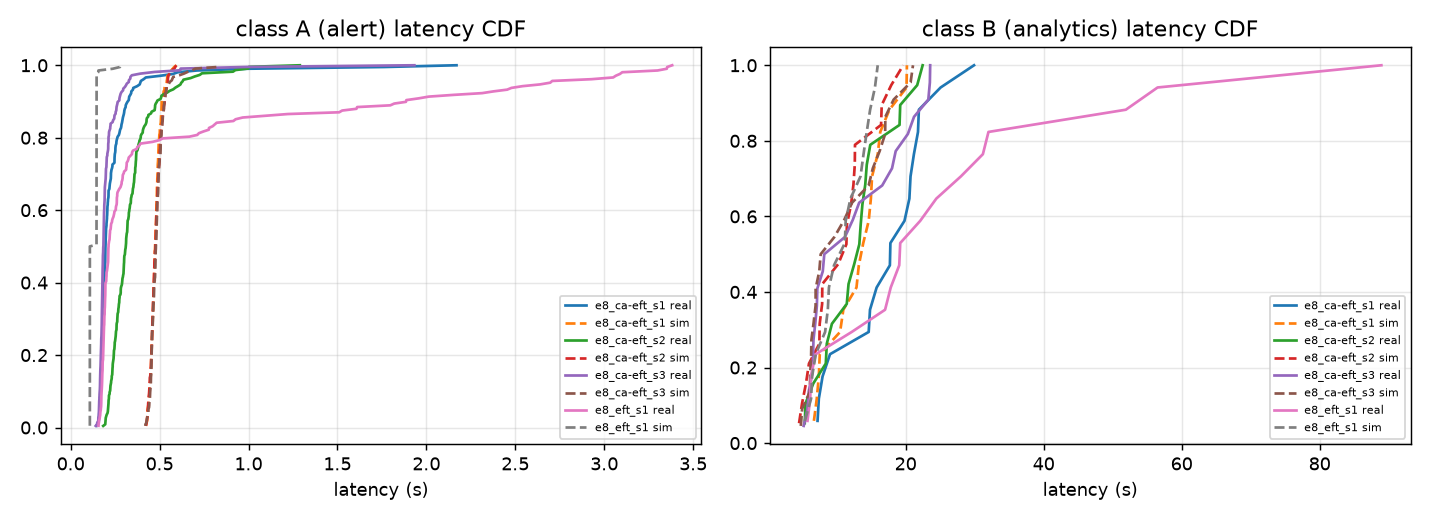
\includegraphics[width=0.8\textwidth]{e9_latency_cdf.png}
\caption{E9: real vs simulated latency distributions for the same job traces.}
\label{fig:e9}
\end{figure}

\subsection{Live demonstration}
The dashboard shows each placement decision with the candidates' estimated finish times and carbon. In a rehearsal with a recorded street video as the camera feed (pedestrians detected at the edge), we exercised a four-fold carbon spike on Mumbai (work stayed off Mumbai), a three-fold rush hour (0.7\% of alerts missed, p95 latency 0.45\,s), a 60-second crash of a Mumbai node (tasks re-queued and re-placed), and a change of the SLA target from 5\% to 1\% ($w$ rose from 0.77 to 0.89 within 30 seconds, without retraining). The rehearsal found and fixed two demo bugs: the worker restarted under systemd and ended the crash after 2.5\,s, and the controller's integral wind-up kept $w$ flat after a target change.

% ================================================================ 8
\section{Discussion and limitations}\label{sec:limits}

\paragraph{Where PACE is strong.} Tight-deadline alerts; heavy load, rush hours, failures and wrong runtime estimates; larger or different topologies, including an unseen grid zone; matching a strong heuristic on deadlines with less carbon; and changing the objective at run time.

\paragraph{Where it is weaker.}
\begin{itemize}
\item \textbf{Large analytics DAGs.} Without the shield, PACE misses more large analytics jobs than CA-EFT (23\% vs 6\% in simulation). The causes are the larger held-out jobs and the missing cross-job cost in the per-decision reward. Next steps: a GNN job encoder and training on larger DAGs.
\item \textbf{Networks far outside training.} With twice the RTT and a third of the bandwidth, PACE misses 17\% against CA-EFT's 1.4\%. On the real testbed, network drift caused the same failure until the online estimate was added.
\item \textbf{Lowest carbon on the testbed.} On real AWS, MERSEM-Balanced used about 15\% less carbon than PACE at $w=0.9$, at many more misses.
\end{itemize}

\paragraph{Threats to validity.}
\begin{itemize}
\item \textbf{Carbon data.} The hourly carbon intensities are synthetic profiles built from real annual means. Free hourly data for the Indian grid zones was not available to us (the Electricity Maps data portal no longer offers free downloads); the code reads Electricity Maps CSVs if they become available. Because the large India--Sweden gap drives most decisions, we expect the ranking to hold, but this is untested.
\item \textbf{Energy is modelled.} AWS exposes no per-VM power, so energy is CPU time times published per-vCPU coefficients times PUE, the same model class MERSEM uses.
\item \textbf{Small testbed.} Six nodes, three seeds per load, one campus network; with six pairs the smallest attainable $p$ is 0.031.
\item \textbf{Re-implemented baseline.} MERSEM's code is not public; we followed the paper and documented every unspecified choice, and we were generous to it (oracle predictor, EFT seeding and fallback).
\end{itemize}

% ================================================================ 9
\section{Conclusion and future work}
PACE turns edge--cloud scheduling into an online, task-level decision taken in about a millisecond by a single preference-conditioned policy. In simulation on the base paper's dataset it misses an order of magnitude fewer deadlines than MERSEM with less carbon, keeps its lead under stress and on most unseen setups, and lets an operator set an SLA target at run time. On a real three-region testbed it missed fewer deadlines than MERSEM in every paired run and matched the best heuristic with 15\% less carbon. Building the testbed was as instructive as the results: it exposed three sim-to-real gaps (dispatch, SMT contention, network drift) that the simulation alone would have hidden.

Future work: a GNN encoder over the job DAG and training on larger DAGs; wider network randomisation and the online network estimate inside training; PPO-Lagrangian as an alternative to the PI controller; real hourly carbon traces with a train-on-one-year, test-on-the-next split; and a longer testbed campaign with more seeds.

\paragraph{Reproducibility.} Code, data, results and run scripts are in the project repository (\url{https://github.com/p-art-dheev/RL-Project}); the commands are in Appendix~\ref{app:repro}.

% ================================================================ references
\begin{thebibliography}{99}\small
\bibitem{mersem} P.~Ramicetty et al. Sustainable graph analytics workload scheduling with evolutionary reinforcement learning in edge-cloud systems (MERSEM). arXiv:2605.13489, 2026.
\bibitem{dataset} S.~A.~Ali Rezaee and S.~Adabi. Jobs (DAG workflow) and tasks dataset. Zenodo, doi:10.5281/zenodo.4667690, CC-BY-4.0.
\bibitem{deeprm} H.~Mao, M.~Alizadeh, I.~Menache and S.~Kandula. Resource management with deep reinforcement learning. \emph{ACM HotNets}, 2016.
\bibitem{deeprm2} Y.~Ye et al. A new approach for resource scheduling with deep reinforcement learning. arXiv:1806.08122, 2018.
\bibitem{decima} H.~Mao et al. Learning scheduling algorithms for data processing clusters. \emph{ACM SIGCOMM}, 2019.
\bibitem{wang2021} J.~Wang et al. Dependent task offloading for edge computing based on deep reinforcement learning. \emph{IEEE Transactions on Computers}, 2021.
\bibitem{abels2019} A.~Abels et al. Dynamic weights in multi-objective deep reinforcement learning. \emph{ICML}, 2019.
\bibitem{yang2019} R.~Yang, X.~Sun and K.~Narasimhan. A generalized algorithm for multi-objective reinforcement learning and policy adaptation. \emph{NeurIPS}, 2019.
\bibitem{ray2019} A.~Ray, J.~Achiam and D.~Amodei. Benchmarking safe exploration in deep reinforcement learning. OpenAI, 2019.
\bibitem{stooke2020} A.~Stooke, J.~Achiam and P.~Abbeel. Responsive safety in reinforcement learning by PID Lagrangian methods. \emph{ICML}, 2020.
\bibitem{wiesner2021} P.~Wiesner et al. Let's wait awhile: how temporal workload shifting can reduce carbon emissions in the cloud. \emph{ACM/IFIP Middleware}, 2021.
\bibitem{edgecloudsim} C.~Sonmez, A.~Ozgovde and C.~Ersoy. EdgeCloudSim: an environment for performance evaluation of edge computing systems. \emph{FMEC}, 2017.
\bibitem{ppo} J.~Schulman et al. Proximal policy optimization algorithms. arXiv:1707.06347, 2017.
\bibitem{ccf} Cloud Carbon Footprint. Methodology (power coefficients per vCPU, PUE). \url{https://www.cloudcarbonfootprint.org/docs/methodology}.
\end{thebibliography}

% ================================================================ appendix
\appendix
\section{Reproducing the results}\label{app:repro}
\begin{small}
\begin{verbatim}
python -m pace.rl.train --minutes 45 --workers 6          # train (optional)
python -m experiments.run_sim --exp all --seeds 10 --procs 6
python -m experiments.plots                               # E1-E5 tables and figures
python -m experiments.run_sim --exp E6 --seeds 10 --procs 12
python -m experiments.e6_report                           # E6 report and figure
python -m testbed.aws up --wide                           # real testbed (AWS credit)
python -m testbed.local --edges 2                         # edge workers, own terminal
python -m testbed.calibrate
python -m experiments.run_testbed --methods pace-shield,pace,mersem,ca-eft,eft \
       --minutes 6 --seeds 3
python -m experiments.testbed_report                      # real-AWS tables
python -m experiments.sim2real                            # E9
python -m testbed.aws down
\end{verbatim}
\end{small}

\end{document}
